\documentclass{beamer}
\usepackage{stmaryrd}
\usepackage{amsthm}
\usepackage{amssymb}
\usepackage{amsmath}
\usepackage{algorithm2e}
\usepackage{hyperref}
\usepackage[french]{babel}
\usepackage{color}
\usepackage{tikz}
\usetikzlibrary{automata, arrows.meta, positioning}

\usetheme{Boadilla}
\usecolortheme{seahorse}

\newtheorem{proposition}{Proposition}
\newtheorem{thm}{Théorème}

\title{Transducteurs et machines de Moore et Mealy}

\author{José et Aimeric}

\begin{document}

\frame{\titlepage}

\begin{frame}
    \frametitle{Table des matières}

    \tableofcontents

\end{frame}

\AtBeginSection[ ]
{
    \begin{frame}{Table des matières}
        \tableofcontents[currentsection]
    \end{frame}
}

\section{Transducteurs finis}

\subsection{Définitions}


\begin{frame}{Définition des transducteurs}
    \begin{definition}
        Un transducteur fini est un 6-uplet $T = (\Sigma, \Gamma, Q, I, F, \delta)$ où
        \begin{itemize}
            \item $\Sigma$ est l'alphabet d'entrée (fini)\\
            \item $\Gamma$ l'alphabet de sortie (fini)\\
            \item $Q$ l'ensemble des états (fini)\\
            \item $I \subset Q$ l'ensemble des états initiaux
            \item $F \subset Q$ l'ensemble des états finaux
            \item $\delta : Q \times \Sigma_{\varepsilon} \times \Gamma_{\varepsilon} \longrightarrow \mathcal{P}(Q)$ est
            la fonction de transition non déterministe
        \end{itemize}
    \end{definition}
\end{frame}

\begin{frame}{Définition des transducteurs}
    \begin{definition}
        On définit $[T]$ la relation reconnue par un transducteur fini $T$, définie comme suit :
        \[ \forall (u, v) \in \Sigma^* \times \Gamma^*, u[T]v \Leftrightarrow \exists q \in I, \exists r \in F,
        r \in \delta^*(q, u, v) \]
    \end{definition}
    \vspace*{0.5cm}
    $\delta^*$ est la fonction de transition itérée
\end{frame}

\begin{frame}{Définition des transducteurs}
    \begin{figure}[h]
    \caption{Un exemple de transducteur fini reconaissant la relation de congruence modulo 2}
    \begin{center}
    \vspace*{0.5cm}
    \begin{tikzpicture}[auto]
        \node (q0) [state, initial, initial text= ] {$q_0$};
        \node (q2) [state, below right = of q0] {$q_2$};
        \node (q1) [state, accepting, above right = of q2] {$q_1$};

        \path [-stealth, thick]
        (q0) edge [loop above] node {$\Sigma_{\varepsilon} \mid \Sigma_{\varepsilon}$} (q0)
        (q0) edge node {$\substack{0 \mid 0 \\ 1 \mid 1}$} (q1)
        (q0) edge [bend right] node {$\substack{0 \mid 1 \\ 1 \mid 0}$} (q2)
        (q1) edge [bend left] node {$\Sigma_{\varepsilon} \mid \Sigma_{\varepsilon}$} (q2)
        (q2) edge [loop below] node {$\Sigma_{\varepsilon} \mid \Sigma_{\varepsilon}$} (q2);
    \end{tikzpicture}
    \end{center}
\end{figure}
\end{frame}

\begin{frame}{Relations rationnelles}
    \begin{definition}
        Soient $R, R' \subset \Sigma^* \times \Gamma^*$ des relations. On pose
        \begin{itemize}
            \item $R \cdot R' = \{ (xx', yy') \mid (x, y) \in R, (x', y') \in R' \}$, la concaténation ou produit
            \item $\displaystyle R^* = \bigcup_{n \geq 0} R^n$ où $R^n$ est la concaténation répétée, et $R^0 =
            \{ (\varepsilon, \varepsilon) \}$
        \end{itemize}
    \end{definition}
    \begin{definition}
        L'ensemble des relations rationelles est défini comme le plus petit ensemble de relations stable par étoile,
        concaténation et union, et contenant $\varnothing$ et les singletons.
    \end{definition}
\end{frame}

\subsection{Premières propriétés}

\begin{frame}{Equivalence}
    \begin{thm}
        Une relation $R$ est rationelle si et seulement si elle est reconnue par un transducteur fini $T$
    \end{thm}

    \begin{proof}
        Exactement le même type de preuve que pour les automates finis et langages rationnels
    \end{proof}
\end{frame}

\begin{frame}{Quelques propriétés de stabilité}
    \begin{proposition}
        L'inverse d'une relation rationnelle est rationnel. Les projections à droite et à gauche d'une
        relation rationnelle sont des langages rationnels
    \end{proposition}

    \begin{proof}
        Pour le premier, on inverse les étiquettes du transducteur reconaissant la relation. Pour le deuxième, on
        "oublie" les étiquettes de sortie pour en faire un automate.
    \end{proof}

\end{frame}

\begin{frame}{Quelques propriétés de stabilité}
    \begin{proposition}
        L'image d'un langage rationnel par une relation rationnelle est rationnel.
    \end{proposition}
    \begin{proposition}
        La composition de relations rationelles est rationelle
    \end{proposition}

    \begin{proof}
        On peut prouver la première propriété à partir de la deuxième, en considérant l'image de la composition de
        $\{\varepsilon \} \times \mathcal{L}$ et $R$.
    \end{proof}
\end{frame}

\begin{frame}{Composition de deux relations}
\begin{figure}[h]
    \caption{Premier transducteur}
    \begin{center}
    \begin{tikzpicture}[auto]
        \node (q0) [state, initial, initial text= ] {$q_0$};
        \node (q1) [state, right=of q0] {$q_1$};
        \node (q2) [state, accepting, right=of q1] {$q_2$};

        \path[-stealth, thick]
        (q0) edge [loop above] node {$a \mid \varepsilon$} (q0)
        (q0) edge node {$a \mid b$} (q1)
        (q1) edge node {$b \mid \varepsilon$} (q2);

    \end{tikzpicture}

    \end{center}
\end{figure}

\begin{figure}[h]
    \caption{Deuxième transducteur}
    \begin{center}
    \begin{tikzpicture}[auto]
        \node (q0b) [state, initial, initial text= ] {$q_0'$};
        \node (q1b) [state, accepting, below=of q0] {$q_1$'};

        \path[-stealth, thick]
        (q0b) edge [bend left] node {$b \mid a$} (q1b)
        (q1b) edge [bend left] node {$\varepsilon \mid b$} (q0b);

    \end{tikzpicture}

    \end{center}
\end{figure}

\end{frame}


\begin{frame}{Composition de deux relations}
\begin{figure}[h]
    \caption{Le transducteur composition des deux relations} \label{prodRel}
    \begin{center}
    \begin{tikzpicture}[auto]
        \node (q0q0) [state, initial, initial text= ] {$q_0, q_0'$};
        \node (q1q0) [state, right=of q0q0] {$q_1, q_0'$};
        \node (q2q0) [state, right=of q1q0] {$q_2, q_0'$};

        \node (q0q1) [state, below=of q0q0] {$q_0, q_1'$};
        \node (q1q1) [state, right=of q0q1] {$q_1, q_1'$};
        \node (q2q1) [state, accepting, right=of q1q1] {$q_2, q_1'$};

        \path[-stealth, thick]
        (q0q0) edge [loop above] node {$a \mid \varepsilon$} (q0q0)
        (q0q1) edge [loop below] node {$a \mid \varepsilon$} (q0q1)
        (q0q0) edge node [swap] {$a \mid a$} (q1q1)
        (q1q0) edge node {$b \mid \varepsilon$} (q2q0)
        (q1q1) edge node {$b \mid \varepsilon$} (q2q1)
        (q0q1) edge node {$\varepsilon \mid b$} (q0q0)
        (q1q1) edge node {$\varepsilon \mid b$} (q1q0)
        (q2q1) edge node {$\varepsilon \mid b$} (q2q0);


    \end{tikzpicture}

    \end{center}
\end{figure}
\end{frame}


\begin{frame}{Une application}
    Si $L$ est un langage rationnel, alors $\operatorname*{Pref}(L)$ l'est également. On retrouve
    ce résultat très rapidement grâce aux transducteurs.
    \begin{figure}[h]
        \caption{Le transducteur reconaissant la relation $\operatorname*{Pref}$ avec $\Sigma = \{a_1, ..., a_n\}$} \label{transPref}
        \begin{center}
        \begin{tikzpicture}[auto]
            \node (q0) [state, initial, initial text= ] {$q_0$};
            \node (q1) [state, accepting, right=of q0] {$q_1$};
    
            \path[-stealth, thick]
            (q0) edge [loop above] node {$\substack{a_1 \mid a_1 \\ ... \\ a_n \mid a_n}$} (q0)
            (q0) edge node {$\varepsilon \mid \varepsilon$} (q1)
            (q1) edge [loop above] node {$\Sigma \mid \varepsilon$} (q1);
        \end{tikzpicture}
        \end{center}
    \end{figure}
    Ainsi $\operatorname*{Pref}(L)$ est simplement l'image de $L$ par une relation rationelle, donc rationnel
\end{frame}

\begin{frame}{Non stabilité de l'intersection}
    Les relations suivantes sur $\{a\}^* \times \{a, b\}^*$
    \begin{equation*}
        \begin{split}
            R_{l} &= \{ (a^n, w) \mid w \in \Gamma^*, n \in \mathbb{N}, |w| = 2n \}\\
            R_{b} &= \{ (a^n, w) \mid w \in \Gamma^*, n \in \mathbb{N}, |w|_b = n \} 
        \end{split}
    \end{equation*}
    sont rationelles. Pourtant
    \[ \{ (a^n, a^nb^n) \mid n \in \mathbb{N} \} = R_l \cap R_b \cap (\operatorname*{Pref})^{-1}\]
    n'est pas rationelle
\end{frame}

\subsection{Quelques problèmes liés aux transducteurs}

\begin{frame}{Indécidabilité de l'équivalence}
    \begin{thm}
        Le problème d'équivalence entre deux transducteurs finis est indécidable
    \end{thm}
    \begin{proof}
        On peut reformuler Post ainsi : étant donné deux morphismes $g, h: \Sigma^* \rightarrow \Gamma^*$, existe-t-il
        un mot $w \in \Sigma^* \neq \varepsilon$ tel que $g(w)=h(w)$ ?\\
        On peut ensuite construire le transducteur qui implémente la relation $(x, (\Gamma^*\backslash \{g(x)\})\cup 
        (\Gamma^* \backslash \{h(x)\}))$, qui implémente la relation $\Sigma^*\times \Gamma^*$ si et seulement si il n'y
        a pas de solution.
        
    \end{proof}
\end{frame}

\begin{frame}{Construction du transducteur.}
    \begin{figure}[h] 
        \caption{Le transducteur qui à un mot $x$ associe $\Gamma^* \backslash \{h(x)\}$} \label{autoG-h}
        \begin{center}
        \begin{tikzpicture}[auto, node distance = 1.4cm]
            \node (q0) [state, initial, initial text= ] {$q_0$};
            \node (q1) [state, accepting, above= of q0] {$-$};
            \node (q2) [state, accepting, right= of q0] {$\neq$};
            \node (q3) [state, accepting, below= of q0] {$+$};
    
            \path[-stealth, thick]
            (q0) edge [loop left] node {$l \mid h(l)$} (q0)
            (q0) edge node {$\Sigma \mid \varepsilon$} (q1)
            (q1) edge [loop above] node {$\Sigma \mid \Gamma_\varepsilon$} (q1)
            (q0) edge node {$\substack{l \mid v \\ \mid v \mid = \mid h(l) \mid \\ v \neq h(l)}$} (q2)
            (q2) edge [loop right] node {$\Sigma_\varepsilon \mid \Gamma_\varepsilon$} (q2)
            (q0) edge node {$\varepsilon \mid \Gamma$} (q3)
            (q3) edge [loop below] node {$\Sigma_\varepsilon \mid \Gamma$} (q3);
        \end{tikzpicture}
        \end{center}
    \end{figure}
\end{frame}

\begin{frame}{Décider de la fonctionnalité}
    \begin{thm}
        Le problème de savoir si un transducteur implémente une fonction (chaque élement n'a qu'une image) est décidable.
    \end{thm}
    \begin{proof}
        Il suffit de tester toutes les images à moins de $O(n^2)$ transitions : s'il existe un mot avec deux images différentes,
        on peut montrer qu'il existe un couple d'images différentes à moins de $O(n^2)$ transitions.
    \end{proof}
\end{frame}

\section{Machines de Moore et Mealy}

\subsection{Machines de Moore}

\begin{frame}{Définition}
    Il s'agit d'un cas particulier de transducteurs finis, ou l'étiquette de sortie ne dépend que de l'état
    courant et où les étiquettes d'entrée sont déterministes
    \begin{definition}
        Une machine de Moore $\mathcal{M}$ est un $7$-uplet $(\Sigma, \Gamma, Q, q_0, F, \delta, \lambda)$ où
        \begin{itemize}
            \item $\Sigma$ est l'alphabet d'entrée
            \item $\Gamma$ l'alphabet de sortie
            \item $Q$ l'ensemble fini des états
            \item $q_0$ l'état initial
            \item $F \subset Q$ les états finaux
            \item $\delta : Q \times \Sigma \rightarrow Q$ la fonction de transition déterministe
            \item $\lambda : Q \rightarrow \Gamma$ la fonction de sortie
        \end{itemize}
    \end{definition}
\end{frame}

\begin{frame}{Définition}
    
\begin{figure}[h]
    \caption{Un exemple de machine de Moore}
        \begin{center}
        Machine de Moore qui note chaque occurrence de la séquence $101$ (tout les états sont acceptants)\\
        \begin{tikzpicture}[auto, node distance = 1.5cm]
            \node (q0) [state with output, initial, initial text= ] {$q_0$ \nodepart{lower} $0$};
            \node (q1) [state with output, right= of q0] {$q_1$ \nodepart{lower} $0$};
            \node (q2) [state with output, right= of q1] {$q_2$ \nodepart{lower} $0$};
            \node (q3) [state with output, below= of q2] {$q_3$ \nodepart{lower} $1$};

           \path[-stealth, thick]
            (q0) edge [loop above] node {$0$} (q0)
            (q0) edge node {$1$} (q1)
            (q1) edge [loop above] node {$1$} (q1)
            (q1) edge node {$0$} (q2)
            (q2) edge [bend left] node {$0$} (q0)
            (q2) edge [bend right] node {$1$} (q3)
            (q3) edge [bend right] node {$0$} (q2)
            (q3) edge node {$1$} (q1);
        \end{tikzpicture}
    \end{center}
\end{figure}
\end{frame}

\begin{frame}{Algorithmes de Pattern Matching}
    On peut reformuler certains algorithmes de pattern matching comme le calcul d'une machine de Moore.
    C'est le cas par exemple de l'algorithme d'Aho Corasick, ou KMP.

    \begin{figure}[h]
        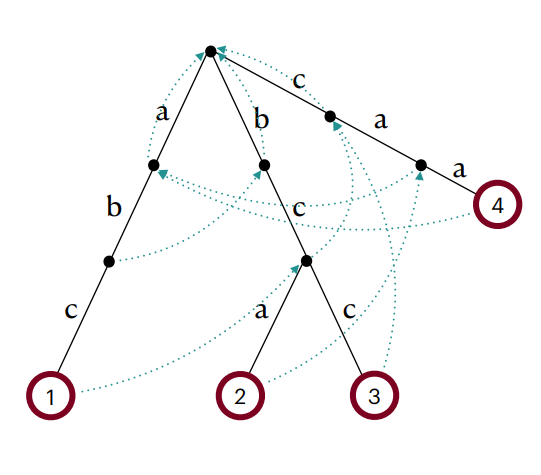
\includegraphics[width = 0.5\textwidth]{Arbre Aho-Corasick.png}
        \\
        Image volée du cours de Tatiana
    \end{figure}
\end{frame}

\subsection{Machines de Mealy}

\begin{frame}{Définitions}
    \begin{definition}
        Une machine de Mealy est un transducteur déterministe sans $\varepsilon$ transition. Il s'agit de la même
        définition que pour les machines de Moore mais où $\lambda : Q \times \Sigma \rightarrow \Gamma$
    \end{definition}
\end{frame}

\begin{frame}{Exemple}
    \begin{figure}[h]
        \caption{Un exemple de machine de Mealy réalisant le ou exclusif de deux entiers}
            \begin{center}
            \begin{tikzpicture}[auto, node distance = 2cm]
                \node (q0) [state, initial, initial text= ] {$q_0$};
                \node (q1) [state, above right= of q0] {$q_1$};
                \node (q2) [state, below right= of q0] {$q_2$};

    
               \path[-stealth, thick]
                (q0) edge node {$0 \mid 0$} (q1)
                (q0) edge node {$1 \mid 0$} (q2)
                (q1) edge [loop right] node {$0 \mid 0$} (q1)
                (q2) edge [loop right] node {$1 \mid 0$} (q2)
                (q1) edge [bend left] node {$1 \mid 1$} (q2)
                (q2) edge [bend left] node {$0 \mid 1$} (q1);
            \end{tikzpicture}
        \end{center}
    \end{figure}
\end{frame}

\subsection{Equivalence Moore/Mealy}

\begin{frame}{Equivalence}
    \begin{thm}
        Pour toute machine de Mealy il existe une machine de Moore équivalente et réciproquement
    \end{thm}
    \begin{proof}
        Pour le sens réciproque, il suffit d'ajouter en étiquette de sortie les étiquettes de l'état vers lequel la transition est faite.
        Pour le sens direct : on clone chaque état $|\Gamma|$ fois (on se place sur $Q \times \Gamma$). Puis pour chaque transition $p \rightarrow q$ d'étiquette
        de sortie $b$, on crée la transition $(p, c) \rightarrow (q, b)$ pour $c \in \Gamma$. De plus on pose $\lambda(q, c) = c$
    \end{proof}
\end{frame}

\subsection{Propriétés algébriques}

\begin{frame}{Semi-groupes}
    \begin{definition}
        Soit $G$ un ensemble muni d'une loi de composition interne $\cdot$. Si $\cdot$ est associative, on appelle $G$ un demi-groupe.
    \end{definition}

    \begin{definition}
        Si $(G, \cdot)$ est un demi-groupe et $A \subset G$ un ensemble fini de générateurs, on peut définir son taux de croissance
        $\gamma : \mathbb{N} \backslash \{0, 1\} \rightarrow \mathbb{N}$ de la façon suivante : pour $n \geq 2$, $\gamma(n)$ est le nombre d'élements
        de $G$ étant produits de $n$ générateurs mais n'étant pas soi même un générateur. En d'autres termes
        \[ \gamma(n) = |\{ g_1 ... g_n \mid g_1, ..., g_n \in A \} \backslash A| \]
    \end{definition}
\end{frame}

\begin{frame}{Exemples de taux de croissance}
    Le semi groupe $\Sigma^*$ avec $\Sigma$ un alphabet fini a un taux de croissance exponentiel (le nombre de mots à $n$ lettres est exponentiel en $n$).
    \\~\\
    Le demi groupe libre $\mathbb{N}^k \backslash \{0\}$ a un taux de croissance polynômial lui
\end{frame}

\section*{Fin}

\begin{frame}{Fin}
    
\end{frame}

\end{document}